\chapter{Results}

After performing a thourough analysis on the gathered scientific papers, we came up with the categorization criteria presented in chapter 3. The contribution type criterion contains the categories 
of tool, framework and algorithm. The tools represent a set of tasks performing different processes in order to achieve a target functional goal. Also, we consider as framework a technique
that uses both different methodologies and also tools to perform the requested task. Finally, we have the algorithm type which is simply the proposal of an algorithm. The reviewed papers have been 
mapped to those types and are presented in more detail in the following sections. \\

The next criterion is the Software Testing Stage. We identified papers which refered to a varitey of phases such as Requirement Analysis, Test Planning, Implementation and also 
Reporting. As we can see, we have found applications concerning a big part of the overall Testing lifecycle. As far as the Testing Type, we have made two kind of categorizations here. 
The first one is Manual and Automated testing, since they are both two popular test types of major significance. We next categorized the approaches based on Integration, Acceptance and Crowdsourced testing. 
However, we also encountered many papers that do not set any limilation to the applicable testing type and, thus, provide more flexibility to that part. Another criterion we indentified is the input type of 
the proposed approach. Some of the most frequent types we found is that of NL test case descriptions, use case specification documents and also test case code. We further analyze these types at the 
corresponding section. As expected, we also refer to the output type as another criterion with the most common ones being the executable code, different tyes of models or diagrams (e.g. Use case/UML diagrams) and 
others. An interesting part of this criterion that we further analyze is that several approaches generate outputs which can then be provided as input to other tools or processes in general. Last but not least, we 
have the NLP Techniques criterion where we analyze in detail the identified NLP methods used on the papers. We study that section by separating it into two categories which are techniques refering to Natural 
Language Understanding and techniques refering to Natural Language Generation. The Natural Lnaguage Understanding component also contains a small section where we present different statistical NLP measures which 
are also used in the reviewed studies.\\

In this chapter, we present the results of our Systematic Literature Review and the study of the papers identified. We separately refer to 
each criterion individually by commenting and making a short reference to the results found. In some sections and always depending on the criterion, we further analyze any 
techniques or practices encountered. 

\section {Contribution Type}
After reviewing all of the papers, we ended up with several contribution types proposed in their context. At this point, we should note that some papers 
proposed more than one types so some of them are included into more than one categories. \\

The first and most encountered contribution type is that of a method technique. This type includes any proposal of approaches, processes, techniques and any 
other alternative way of performing a certain task. We grouped them all into this category since they all somehow refer to something very similar. Specifically, 20 of the
studied papers suggest such an approach of that type. 9 out those 20 papers (45\%) propose a way for generating test cases automatically from different input types, like 
use case specification and funtional requirement documents. Motwani et al \cite{8812070}, for example, present Swami which is a language-agnostic test case constructor 
based on Javascript code templates and the ECMA-262 Standard. Swami generates test case code based on the code documentation and software specifications provided. Moreover, 
Nogueira et al \cite{nogueira2015automatic} propose an event flow for test case generation from input provided in a Control Flow Language. This flow consists of several other 
processes (e.g. translation of use case descriptions) that contribute to the achievemennt of the overall goal of the proposal. \\

Another significant contribution type we distinguished is that of a tool. 14 of the studied papers suggest some sort of tool for the ease of different software testing processes. 
Some of those tools are part of the overall approach, whereas others are the main focus of the study. Some of them target the test case execution process, others focus on test case 
generation or even other areas like defects prevention and requirement analysis facilitation. Pedemonte et al \cite{pedemonte2012towards} present an approach to convert manual 
functional tests into a state ready for automatic execution by using Machine Learning methods to process textual information. This is a semi-automatic approach since in cases 
of textual information ambiguity, the user is prompted to interact with the tool to resolve the issue and provide the answer required to continue with the process. Another 
considerable approach is the CTRAS tool created by Hao et al \cite{8811987} which aims at the summarization of duplicate test reports in oprder to make them easily understandable 
by developers. The tool idenitfies similarities in both textual information and screenshots and comprehensibly presents them into a single report. \\

Several other papers focused on developing a Framework to achieve their goal. Some of them refer to the topic of test case generation while others 
emphasize on the earlier stage of requirement analysis and transformation. Lafi et al \cite{9491761} created a framework which consists of different other 
processes in order to generate test cases. First of all, the use case descriptions are being processed in order to create a control flow graph and an NLP table of the 
system under test. Based on those, test paths are then generated which they will finally lead to the test case code. As far as the requirement analysis phase 
is concerned, Viggiato et al \cite{viggiato2022using} created a framework in order to help testers improve the test cases they create. This framework 
accepts test cases in natural language as input and then provides recommendations and proposed changes. More specifically, it can provide recommendations 
for the improvement of the terminology of the test cases, it can identify potentially missing test steps from those test cases and lastly, it can 
prevent test case duplicates since it is able to identify similar test cases with the one which is currently being analyzed. All of the above three 
outputs contribute immensely to the proper and effective forming of test cases by making the testers' job much easier. \\

The last contribution type spotted is the proposal of some sort of strategy. This might be a certain way of handling or working on a specific process which 
could include the use of some specific method or tool. Yet again, the papers we identified serve different kinds of purposes on different stages 
of testing. Wong et al \cite{wong2015dase} propose DASE, a path pruning strategy which aims to improve test case execution and bug detection. It can also prevent 
defects and increase test coverage. It operates by extracting input constraints from program documentation in order to guide and form test execution paths. 
Moreover, Tahvili et al \cite{10.1145/3195538.3195540} proposed a strategy which, given test specifications in natural language, idntifies relationships 
between those test cases and finally, generates a series of proposed test case scheduling strategies for execution. This is great way to effectively 
prioritize the test case execution process and optimize test case execution. \\

After the analysis of the identified contribution types of the papers studied, we notice that the majority of scientific contributions revovle around 
the proposal of a technique or method of performing a process. This is not something unexpected. Software Testing consists of any major processes, like 
test case generation, test planning, defect prevention and others, which shape all together the overall purpose of this knowledge area. Thus, the fact that 
many researchers and people interested in the field have figured out ways to enhance those methods makes a lot of sense. They have achieved 
that by proposing new tehniques that be integrated to these processes and give out great results.

\section {Software Testing Stage}
Another aspect of the papers we studied that we are intersted in is the Stage of the Software Testing Lifecycle to which they apply. Some of the approaches we found refer to 
the Requirement Analysis phase, others to the Implementation and Development, Execution etc. The first one we will comment here is the Requirement Analysis. Almost 18\% of the studies 
come up with a proposal regarding that stage and they target to enhance the processing of the test requirements and specifications. This procedure happens before the construction 
of the test cases of any form and it is a critical stage which many times determines the overall outcome of the testing cycle. Thus, it is of major importance to effectivelly 
perform the Requirement Analysis for the optimal result. \\

Sainani et al \cite{reqclass}, for example, propose a method technique which idenitfies and classifies requirements from software engineering contracts. These documents contain all 
the necessary information about the product to be developed, and therefore tested, with the desired characteristics and specifications being a part of them. The developed approach 
analyzes the contract document using different NLP techniques, which we will discuss in a further section, and outputs the different requirements of the product as well as their type. 
The output might add important information regarding the product's architecture or the importance of each feature. Based on that, developers and testers get a clear overview of what 
is worth to be tested more and also the parts that need more attention during the development and testing. This method refers to very early steps on software testing. However, 
this does not mean that such a process is not significant for a successfull testing cycle. On the contrary, it sets a concrete base for all the other stages that follow. \\

Equal importance to the Requirement Analysis stage is given by Femmer et al \cite{femmer2017rapid}. They propose a tool called Smella, which identifies Requirement Smells inside 
Requirement documents. At this point, it is worth mentioning what Requirement Smells actually are. Code smells are parts of code that need to be somehow changed in order to enhance 
its structure, complexity or comprehension \cite{fowler2018refactoring}. Consequently, Requirement Smells represent spots of Requirement Documents which need to be modified in a 
certain way in order for the product's specifications to be stated with the optimal way. For example, in a certain document it is possible to have the same requirement expressed in 
a different way. This might happen due to syntax mistakes or overall use of complex syntax in the document, which makes comprehension a harder task for the reader. This is 
the job of the Smella tool. By making good use of different NLP techniques and incorporating them into the tool, the authors managed to perform the processed described above. \\

The next stage we will refer to in this section is Software Test Planning which contains tasks like Effort Estimation and the overall planning of the roadmap of the testing 
process. Yang et al \cite{9617598} propose a method called DivClass which aims to define the optimal prioritization of test reports inspection in Crowdsource Testing. This testing type 
is covered in a next section of this chapter, so we will not further explain it here. The proposed method initially performs numerous natural language processing tasks to transform the 
test report dataset it accepts as input. Then, the similarity of those test reports is calculated and finally, based on that, the inspection priority of each one is determined. This is a 
short description of the overall method. We perform detailed reference to the different NLP techniques in Section 4.6. This approach can benefit the Software Testing process since it can 
reduce the time spent on the inspection of test reports which are not that critical or that they don't contain high importance information. On the contrary, substantial amount of time 
can be spent on inspecting test reports of higher priority. Another method which targets to make Software Testing faster is the one proposed by Tahvili et al \cite{8051381}. Their approach 
predicts the execution time of manual test cases based on their textual specifications and also on historical data from previously executed test cases. Undoubtedly this approach has a lot 
to offer to the software testing community since it enhances the manual test case execution process which most of the times it ends up requiring the most amount of time to be completed. Taking 
into account that the tester now knows the approximate execution time of the test cases, it is easier for him/her to plan the overall test cycle and create the expected timetable. \\

The testing stage which gathers the majority of the attention in the scinetific literature is the implementation/development stage. That is when the test cases are created and the whole testing 
project comes to life. At this point, it is worth mentioning that almost the 70\% of the papers studied refer to that stage in some way. Because of that, we have a plethora of approach types each 
targeting a different issue. A very common task we frequently came across is the one of test case generation, usually from Requirement Documents expressed in Natural Language. Kamalakar et all 
\cite{kamalakar2013automatically}, for example, created a tool called Kirby which generates test case code from textual Requirement Specifications. Code pieces of the System Under Test 
can be also used in order for the tool to better understand the structure and semantics. However, the framework proposed by Lafi et al \cite{9491761} in order to perform the same task is different. 
This approach uses the Use Case Description of the Use Case Diagram expressed in UML. It is obvious that there is a variety of alternatives that achieve the same goals, which is the test case generation. 
Though this is not the only one we identified at the implementation stage. Viggiato et al \cite{viggiato2022using} propose a framework which aims at improving manual test case descriptions. More specifically, 
this approach accepts the test cases expressed in natural language and generates recommendations for the improvement of those descriptions. The framework recommends test case terminology improvements, 
identifies possible missing steps from those test case and it is also capable of finding potential test cases that already exist in the test code and which are similar to the one provided as input. This 
is a very powerfull approach which makes the test case implementation a piece of cake. Developing test cases based on clear, complete and comprehensive descriptions eliminates the possibility of 
mistakes and makes the whole process much faster. \\

Some of the papers we studied aim to also enhance the stage of test case execution. Pedemonte et al \cite{pedemonte2012towards} created a tool which converts manual test cases into automated ones. 
In their analysis, they emphasize on the importance of the automatic test case execution and that is why they pursuited the implementation of that task. Their approach has the ability of accepting user 
guidance if necessary, but 70\% of the test cases on which they evaluated the tool converted automatically to automated test steps without user guidance. Consequently, we see that the execution stage is also 
considered a significant one for the sucessfull completion of the Software Testing process. \\

After analyzing the testing stages on which the studied papers refer to, we should make a short reference to a less popular issue of the testing world which is that of test report manipulation. Some of the studies 
we encountered, develop approaches that aim to transform test code and outcomes into a more human-friendly format. Hao et al \cite{8811987} created a tool which not only identifies duplicate reports, but it also 
summarizes their content into a more comprehensive report. This process also happens on bug reports. On the other hand, Gonzalez et al \cite{10.1145/3283812.3283819} implemented a tool which performs a process 
opposite to what we have encountered so far in this review. The created tool converts JUnit Assertions into text written in English. Goal of this approach is to contribute to the maintenability, understandability 
and analysis of test code by reducing the existence of complex and difficult to explain code.

\section {Software Testing Type}
In this section of our analysis, we focus on the test type that each approach refers to. The first kind of categorization we will perform is based on the two wide groups of manual and automated tests. 
Those two testing approaches are widely used in software testing with each one of them serving a different purpose. Manual Testing is a well-established technique where the tester interacts with the 
application in order to validate and ensure it functions as expected and according to requirements. He performs the steps described in the test cases by manually executing them. However, this is an 
extremely expensive process and requires a big amount of resources with time and money being some of them. This gap fills the use of Automated Testing, where important stages like test generation and execution 
are performed automatically. This process significantly decreases the amount of time needed to test the product and that is the reason why Automated Testing is widely used in Agile development where 
software releases are continuous and more frequent. Moreover, a big number of papers did not set any restrictions on the testing type to which they refer and they usually include improvement recommendations for 
the overall testing process. The results of the analysis based on Testing Type are also presented in Figure 1.\\

\begin{figure}[h]
    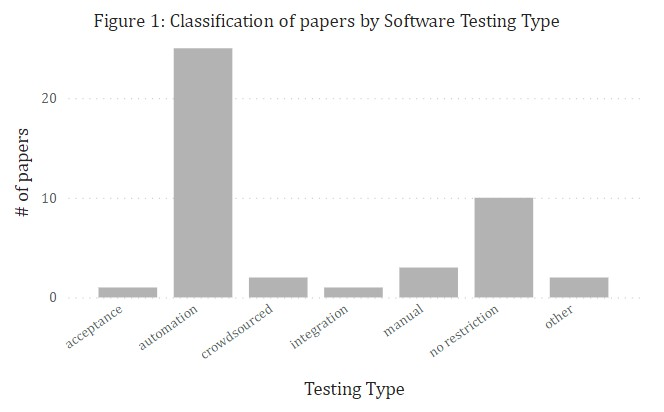
\includegraphics[width=15cm]{testing_type_diagram.jpg}
    \centering
\end{figure}

We will firstly refer to the papers that contribute to the manual testing domain. A significant fact we notice from studying the approaches is that they refer to different phases of testing. With manual 
testing alone being a category of major importance, it is somehow reasonable for it to concern a big part of the software testing community. The Toucan4Test tool proposed by Zhang et al \cite{zhang2014systematic} facilitates 
the process of test cases forming and creation from requirements in natural language. More specifically, this approach automatically generates the test cases from specification documents in order for them to be manually 
executed from the testers. This entails that the above process outputs test cases in a comprehensive format which the executor can easily understand and that he can follow the test steps without any trouble. On 
the other hand, Tahvili et al \cite{8051381} focus on manual test planning. Since we also referred to this approach in a previous section of this chapter, here we will shortly recall the context of the proposed method. 
The authors proposed a technique which predicts the execution time of manual test cases. Such an ability is crucial for the optimized manual test execution since this is a very time consuming process. Thus, 
an effective scheduling of the test cases that are to be executed is more than important.\\

Although manual tests are a widely used testing method, automated testing has significantly grown the past few years and it continues to develop. This is also obvious from the fact that 25 out of all the papers studied 
in this review refer to this testing method. Consequently, these approaches correspond to various contribution types and testing stages. They refer to the automatic creation, forming and execution of test cases from 
different sources like requirement documents or use case diagrams. At this point, we should note that the majority of those techniques are applied during the implementation stage. One such example is the Litmus tool 
created by Dwarakanath et al \cite{litmus} which generates test cases from requirement documents without imposing any restrictions to the input language format or syntax. The tool follows a five step process. After it 
verifies that a sentence of the document is testable, the processing and generation procedure of the test case begins. A similar tool was developed by Rane et al \cite{rane2017automatic}. However, in that case the 
authors focused on optimizing the software testing process during Agile software development.\\

Apart from the above two big groups of manual and automated tests, we identified several other more specific testing types according to which we can further characterize some of the studied approaches. Those types are 
acceptance, integration and crowdsourced tests. The goal of acceptance tests is to determine whether the application meets functionality and usability criteria \cite{artoftesting}. These tests are performed by the 
end users of the application. An example of such approach we identified in the papers is the one proposed by Wang et al \cite{wang2020automatic} which targets the automatic generation of acceptance test cases and also, 
their automatic execution. Thus, the manual effort required is significantly reduced. Moving on to the Integration Testing type, it aims to verify that all the system modules and units communicate correctly 
to perform the functionality required \cite{leung1990study}. This testing type is performed after Unit Testing which, on the other hand, tests each module of the application separately. The technique proposed by Rajaraman et 
al \cite{9197868} targets Integration Testing. More specifically, goal of the approach is to identify interconnections and dependencies between different components of an application in order to optimize Integration Testing. 
The dependencies are determined based on the frequency of use and the importance of each component. Such characteristics exist in the application log files which are also the input of the proposed approach of 
the specific paper.\\

The third testing type we will talk about in this section is Crowdsourced Testing. Crowdsourced Testing has been growing in popularity during the last few years with many platforms having already 
been developed to serve that purpose, such as CrowdSprint\footnote{https://crowdsprint.com/crowdsourced-testing/} and TestBirds\footnote{https://www.testbirds.com/services/quality-assurance/}. 
In Crowdsourced Testing, test tasks are available online for anyone who is willing to perform them and test various software products. When the test task is completed, a test report is submitted 
describing the software's behavior \cite{cui2017should}. A paper that focuses on this testing type is one we have previously encountered in this chapter written by Yang et al \cite{9617598}. The authors 
propose a method called DivClass which prioritizes the test reports coming from Crowdsource testers. Also, similar reports are identified and combined into a signle report for more effective management 
of time during test report inspection.\\

Having expanded on the Software Testing Type characteristic of this review, we notice an overall tendency of the scientific community mainly towards Automation Testing approaches and methods to further 
evolve this practice, which is currently gaining a lot of attention. The next major field of interest is Manual Testing, an older and well established method which continues to being a part of the Software 
Testing process. Lastly, we came up to a number of papers which emphasized on a more specific testing type without making distinctions regarding the above categories of Automated and Manual tests. Such test 
types are Integration, Acceptance and Crowdsourced Testing. However, the approaches proposed there can be utilized during both automated and manual testing.

\section{Input Type}
The input type of the studied approaches is another significant criteria based on which we will characterize them. During our analysis, we notice 
that the nature of the input that each method accepts varies from being some sort of test case code, requirement and use case documents. However, the 
majority of the inputs represent information written in natural language.\\

We will start by referring to the approaches that need test case code in order to perform the functionallity required. The tool proposed by Gonzalez et al \cite{10.1145/3283812.3283819} accepts 
as input the test code of the system under test and in particular the part of it which contains the assertions performed to check different parts of the testing 
process. After the JUnit assertions have been provided to the tool, then a summary of the code is generated. More specifically, the assertion code 
is translated into natural language statements in English. That way, the test case code obtains a comprehensive format and the maintenance 
of the test cases becomes way easier and faster. Another approach which has test case code as one of its accepted inputs is the one proposed by 
Kamalakar et al \cite{kamalakar2013automatically} which we have previously referenced again in this chapter. The goal of the approach is the generation 
of test cases from the textual descriptions of the software's functionallity. However, code pieces of the software under test can be also provided as input 
to the approach in order for the tool to better understand the behavior and expected functions of the application that is being tested.\\

A very frequent input type we came across during our analysis is that of test case descriptions written in natural language. The method proposed 
by Kirinuki et al \cite{9609160} aims to facilitate the maintenance of the automated test scripts where the identification of web elements on 
web pages is necessary. In a web application elements like buttons, text input fields etc. tend to change as the application develops. That 
means that the corresponding test scripts need to constantly adapt to the new changes. However, such a process is very time consuming and 
not effective. Thus, the authors move towards script-free testing by proposing a technique where testing is performed through executable test 
cases in natural language with no need to create test scripts. Arruda et al \cite{arruda2020automation} on the other hand, developed a strategy 
for test script generation which accepts as input the textual test case descriptions. This strategy generates reusable code and is also able 
to adapt and integrate with other test generation frameworks for even better results.\\

The use cases and user stories of the system under test is another common input type referenced into the papers studied. That information can be provided through different forms like diagrams or 
textual documents. However, we noticed that textual descriptions outweigh the rest of the accepted input formats. The method proposed by Nogueira et al \cite{nogueira2015automatic} is one of the many which 
aim at the automatic test case generation. However, its accepted input type is the application's use cases written in a Controlled Natural Language (CNL) proposed by the authors. As stated in the paper, CNL 
is a subset of English that can be processed and translated into a formal language with possibly a different format \cite{nogueira2015automatic}. On the other hand, the approach of Mulla et al \cite{mulla2020potent} 
incorporates the user stories into software testing by specifically focusing on Agile practices. This approach exposes the importance of user story artifacts in the whole Software Testing Lifecycle by 
offering, at the same time, reusability of code, increased test case generation speed and reliability.\\

After the analysis of the different input types of the suggested approaches, we cannot question their variety and diversity. However, there is no doubt that most of them share a common characteristic. The input 
information is usually expressed in natural language in order for the corresponding method or tool to perform the task required. Since the papers we study combine Natural Language Processing Techniques with 
Software Testing, it is more than reasonable for the proposed approaches to make good use of textual information of all sorts. This is another way through which the whole contribution of the NLP knowledge area is evident.

\section{Output Type}
We are now moving on to the output type characteristic based on which we will continue our analysis. The different output types distinguished seem to serve multiple purposes. Several approaches generate 
results ready to be used and to enhance the testing process, whereas others create information which can then act as input into another tool, framework or process. Test reports is another frequently encountered type 
which sometimes is also seen to incorporate bug reporting information.\\

The first output type we will refer to is any form of generated code. The corresponding papers of this output type implement automatic test case generation from different input information and as a result, 
they generate executable test case code. The approach of Mueller et al \cite{inproceedings} does exactly that based on the textual requirements of the application's behavior. This is achieved by firstly 
transforming abstract textual information into a more normalized format (Textual Normal Form --- TNF) and then, the authors make good use of the UML diagram representation where the initial information 
is transferred. The UML diagram is translated into classification trees which finally, generate the output code. At this point, we should note that the generated result uses the SystemVerilog language 
to represent the corresponding outcome. According to Bergeron et al \cite{bergeron2006verification}, ``\emph{SystemVerilog is the first truly industry-standard language to cover design, assertions, 
transaction-level modeling and coverage-driven constrained random verification.}'', meaning that SystemVerilog provides a huge flexibility and support when it comes to working in areas like high-level data types, 
object oriented programming, assertions and others. That way, integration does not act as a barrier when it comes to moving and exchanging knowledge and information related to different areas each.\\

Our analysis now continues with the papers which generate information that can be then provided as input to other processes and frameworks. The method proposed by Li et al \cite{10.1145/3368089.3417067} 
identifies similar test steps by using clustering techniques. The generated output is the created clusters which contain the common test steps. Those clusters can be then taken into advantage in order 
to create or even refactor API test methods. Either by acting as input to another tool or by simply being a useful source of information to the Test Engineer, this approach achieves the development of 
simpler and clean test code.\\

Different forms of models and diagrams is another frequent output type we came across during our analysis. Some of the corresponding approaches refer to the implementation stage, but the number of methods 
that target Test and Requirement Analysis is equally noticeable. Harmain et al \cite{harmain2000cm} developed a tool called CM-Builder which aims at facilitating the process of test analysis. This tool 
accepts textual information regarding the corresponding software's requirements and then formally presents that information into a UML class diagram, consisting of the necessary object classes of the system. 
This class diagram can be then provided to any Test Analyst for further improvement. Thanks to the above process, the overall analysis of the system to be tested is being both enhanced and accelerated. 
Similar is the goal of the MaramaAIC tool developed by Kamalrudin et al \cite{kamalrudin2017maramaaic}. However, the authors focus much more on the textual requirements improvement, thus after the input 
specification documents have been provided to the tool, the generated output is either a model or diagram containing the idenitfied recommendations. Those recommendations can be proposals to provide better consistency, 
completeness and correctness to the requirements.\\

Having concluded our analysis on the output types of the studied approaches, we see that there are two major types which stand out. Those are the executable test code and any form of model or diagram describing 
some type of information. Approaches that generate test code usually aim at the direct implementation and execution of the test cases and have taken up the mission to accelerate the overall testing process. On the 
other hand, papers that propose small and more detailed tools or methods and target the improvement of one specific stage or procedure, provide small but very useful improvements to small steps of the testing process. 
Nonetheless, both of the above directions, effectively and in their own way, enhance the testing journey. A more detailed overview about the studied papers and their matching to 
the above criteria is shown in \hyperref[table2]{Table 2} below.

\begin{longtable}{|p{3cm}|p{1cm}|p{2.5cm}|p{2.8cm}|p{2.5cm}|p{2.5cm}|}
    \caption*{Table 2. List of the studies reviewed by Contribution Type and Software Testing Stage}
    \label{table2}\\
        \hline
        Title & Ref. & Contribution Type & Software Testing Stage & Input & Output\\
        \hline
        A systematic approach to automatically derive test cases from use cases specified in restricted natural languages   & \cite{zhang2014systematic}&  67 & Requirement Analysis & NL Test Case Descriptions &
        Test Case Specifications in RTCM format \\
            \hline DASE: Document-Assisted Symbolic Execution for Improving Automated Software Testing & \cite{wong2015dase} & --& Requirement Analysis & Code Comments and Manual Pages & Detected bugs, Code Coverage results\\
            \hline Extracting and Classifying Requirements from Software Engineering Contracts  & \cite{reqclass} & aaa & Requirement Analysis & Software Engineering Contracts & Architectural Requirements\\
            \hline Determining Software Inter-Dependency Patterns for Integration Testing by applying Machine learning on Logs and Telemetry data
            & \cite{9197868} &  24 & Requirement Analysis & Log Files & Identified Dependences\\
            \hline Processing Natural Language Requirements & \cite{ambriola1997processing} & --& Requirement Analysis & Requirement Document & a Web-based environment aiding in NL requirements gathering  \\
            \hline Rapid Quality Assurance with Requirements Smells   & \cite{femmer2017rapid} & --& Requirement Analysis & Requirement Document & Identified Requirement Smells\\
            \hline CM-Builder: An Automated NL-based CASE Tool  & \cite{harmain2000cm} & --& Requirement Analysis & Requirement Document & UML Diagram in a semantic network\\
            \hline MaramaAIC: tool support for consistency management and validation of requirements  & \cite{kamalrudin2017maramaaic} & --& Requirement Analysis & Textual Requirement Specifications &
            Corrected use case model/diagram\\
            \hline Detecting System Use Cases and Validations from Documents & \cite{6693114} & --& Requirement Analysis & Requirement Document & Detected use cases and rules\\
            \hline Score-Based Automatic Detection and Resolution of Syntactic Ambiguity in Natural Language Requirements & \cite{9240680} & --& Requirement Analysis & Requirement Documents &
            Possible word interpretations and proposal for ambiguity resolving\\
            \hline Crowdsourced Test Report Prioritization Based on Text Classification  & \cite{9617598} & --& Test Planning & Test Report Dataset & Test Reports in recommended order\\
            \hline Towards Execution Time Prediction for Manual Test Cases from Test Specification  & \cite{8051381} & --& Test Planning & NL Test Case Descriptions & Predicted Execution Time\\
            \hline Automatically Generating Tests from Natural Language Descriptions of Software Behavior  & \cite{kamalakar2013automatically} & --& Implementation & NL Test Scenario Descriptions, 
            Code pieces of developed software & Test Case Code\\
            \hline Towards Transforming User Requirements to Test Cases Using MDE and NLP & \cite{allala2019towards} & --& Implementation &User Requirements container (URCon) & Container with 
            annotated user requirements (AnnURCon) \\
            \hline Litmus: Generation of Test Cases from Functional Requirements in Natural Language  & \cite{litmus} & --& Implementation & Requirements Document & Test Case Code\\
            \hline Automation and consistency analysis of test cases written in natural language: An industrial context & \cite{arruda2020automation} & --& Implementation & NL Test Case Descriptions& Test Case Code\\
            \hline NAT2TESTSCR: Test case generation from natural language requirements based on SCR specifications  & \cite{carvalho2014nat2testscr} & --& Implementation & Requirements written in SysReq CNL& Software 
            Cost Reduction Specifications Document\\
            \hline Towards Automatic Functional Test Execution & \cite{pedemonte2012towards} & --& Test Execution & NL Test Case Descriptions & Adjusted Automated Test and Report\\
            \hline Abstract Flow Learning for Web Application Test Generation  & \cite{10.1145/3278186.3278194} & --& Implementation & NL Test Case Descriptions &ML-based trainable test flow generation system \\
            \hline A Natural Language Programming Approach for Requirements-based Security Testing & \cite{mai2018natural} & --& Implementation & NL Test Case Descriptions & Executable Security Test Cases\\
            \hline Automatic Generation of Acceptance Test Cases from Use Case Specifications: an NLP-based Approach & \cite{wang2020automatic} & --& Implementation & User Story, Test Scenario Descriptions &
             Test Case Code\\
            \hline Automatic Generation of Test Cases for Agile using Natural Language Processing & \cite{rane2017automatic} & --& Implementation & NL Test Case Description & Test Case Code\\
            \hline Cluster-Based Test Scheduling Strategies Using Semantic Relationships between Test Specifications & \cite{10.1145/3195538.3195540} & --& Implementation & Test Specifications&
            Test Case Clusters ready for scheduling\\
            \hline Clustering Test Steps in Natural Language toward Automating Test Automation & \cite{10.1145/3368089.3417067} & --& Implementation & NL Test Case Descriptions & Test Case Clusters\\
            \hline Generation of Executable Testbenches from Natural Language Requirement Specifications for Embedded Real-Time Systems & \cite{mueller2010generation} & --& Implementation & Textual 
            Requirement Specifications & SystemVerilog Code\\
            \hline Automated Test Cases Generation From Requirements Specification  & \cite{9491761} & --& Implementation & Use Case Description model & Test Paths, NLP table\\
            \hline Constructing Test Cases Using Natural Language Processing  & \cite{7972390} & --& Implementation & Functional Requirement Document & Test Case Table\\
            \hline NLP-assisted Web Element Identification Toward Script-free Testing & \cite{9609160} & --& Implementation & NL Test Case Descriptions & Test Procedure in NL\\
            \hline NLP-Based Requirements Formalization for Automatic Test Case Generation & \cite{inproceedings} & --& Implementation & Functional Requirements&  Requirements Model\\
            \hline Syntactic Rules of Extracting Test Cases from Software Requirements  & \cite{masuda2016syntactic} & --& Implementation & Functional Requirements & Syntactic Rules for Test Case Generation\\
            \hline Test Case Reuse based on ESIM Model  & \cite{chen2021test} & --& Implementation & New Test Case & Test Cases Similarity\\
            \hline A Linguistic Analysis Engine for Natural Language Use Case Description and Its Application to Dependability Analysis in Industrial Use Cases
              & \cite{sinha2009linguistic} & --& Implementation & Use Case Descriptions & Use Case Description Model\\
            \hline Using Natural Language Processing Techniques to Improve Manual Test Case Descriptions & \cite{viggiato2022using} & --& Implementation & NL Test Case Descriptions & 
            Test Case Improvement Recommendations\\
            \hline A Natural Language Processing (NLP) Framework for Embedded Systems to Automatically Extract Verification Aspects from Textual Design Requirements
            & \cite{anwar2020natural} & --& Implementation & Textual Design Requirements & Verification Assertions\\
            \hline Automatically Generating Precise Oracles from Structured Natural Language Specifications & \cite{8812070} & --& Implementation & Test Case Specifications Document & Test Case Code\\
            \hline On Learning Meaningful Assert Statements for Unit Test Cases & \cite{9283916} & --& Implementation & Test and Focal method context & Assert statements\\
            \hline Building Combinatorial Test Input Model from Use Case Artefacts & \cite{preeti2017building} & --& Implementation & Use Case Specifications & Test Case Model\\
            \hline Automatic generation of test cases and test purposes from natural language & \cite{nogueira2015automatic} & --& Implementation \& Test Execution & CNL Use Cases &Test Case Code\\
            \hline A Fine-Grained Approach for Automated Conversion of Junit Assertions to English  & \cite{10.1145/3283812.3283819} & --& Reporting & Test Case Code Assertions & English text  \\
            \hline CTRAS: Crowdsourced Test Report Aggregation and Summarization  & \cite{8811987} & --& Reporting & Test Report & Textual information and/or screenshots of duplicate tests \\
            \hline Towards the identification of bug entities and relations in bug reports & \cite{li2022towards} & --& Reporting & Bug Reports & Relations between bug entities\\
            \hline Mining Historical Test Logs to Predict Bugs and Localize Faults in the Test Logs & \cite{8812113} & --& Test Planning & Test Logs & Identified Faults\\
            \hline The Potent Combo of Software Testing and NLP & \cite{mulla2020potent} & --& Requirement Analysis& User Stories, Test Scenario Description & Test Case Code\\
            \hline Assisted Behavior Driven Development Using Natural Language Processing & \cite{soeken2012assisted} & --& Implementation & Test Case Code, NL Test Case Descriptions & UML class/sequence diagram\\
        \hline
\end{longtable}

\section{NLP Techniques}
The field of Natural Language Processing (NLP) consists of two different components each referring to a specific task. The first one is Natural Language Understanding (NLU) and the second one is Natural Language 
Generation (NLG) \cite{liddy2001natural, khurana2017natural}. NLU involves the study and processing of text in multiple levels and aspects (e.g. syntactical, morphological etc.), in order to map the given textual 
information into useful representations. \\
NLU contains several steps which actually represent different analysis types \cite{liddy2001natural}. The first kind is Lexical Analysis which has to do with the understanding of a word's structure. 
The content of this analysis represents the Lexicon of the language which is being analyzed and contains a total of words and phrases of this language. Next we have Syntactic Analysis, during which sentences are parsed, 
based also on grammar rules, in order to analyze the relationship between words. Semantic Analysis is another NLP 
step which identifies all the possible meanings of a sentence based on the interaction of each individual meaning of the words comprising it.  For example, the sentence ``I will send a friend to my letter'' will be rejected 
during Semantic Analysis.The next type is Discourse Analysis. This kind of analysis focuses on the meaning of a text which is conveyed by the interaction of the meanings of the different sentences it contains. Lastly, we have 
Pragmatic Analysis where sentences are re-interpreted on their real meaning like, for example, the idenitification of the subject on sentence pronouns like ``him'', ``them'' etc.\\ As far as NLG is concerned, 
it refers to the creation of meaningful texts of different formats based on an input resource. The process consists of three phases which are identifying the goal of the task, planning on how this goal can 
be achieved taking into consideration the available resources and finally, implementing the plan created into text \cite{khurana2017natural}. The majority of the papers studied in this review perform NLU. 
However, very few papers performing NLG were also identified.

\subsection{Natural Language Understanding --- NLU}
We will firstly analyze the techniques used which belong to the NLU component.
Since lexical analysis aims to understand the meaning of each word individually, Part-Of-Speech (POS) tagging is one of those techniques who widely 
contribute to this process. POS tagging is used in the majority of the reviewed papers because it performs a very important task for the text processing 
procedure. Goal of this technique is to assign to each word the part of speech tag to which it belongs. POS tagging distinguishes wheather a word is 
a noun, a verb, an adverb etc. In our case, it is frequently used in user requirements analysis in order to transform them into use cases which finally 
helps generate the required test cases \cite{allala2019towards, wang2020automatic, rane2017automatic, 8812070, preeti2017building, mulla2020potent}. 
Moreover, we also encountered POS tagging being used in proposed methods that focus on bug reporting and ambiguity detection in user requirements. 
Osama et al \cite{9240680}, for example, use it to assign three different types of ambiguites (semantic, syntactic and syntax) to the information identified. \\
However, several authors moved one step further from POS tagging. Specifically, we identified two papers that adopted a slightly altered approach. 
Pedemonte et al \cite{pedemonte2012towards} utilize BIO tagging \cite{ramshaw1999text}. BIO tagging faciliates the process of creating or identifying chunks of words or sentences in a text. 
In contrast to POS, BIO tagging does not assign only one label to a token, but it inserts a prefix to each token's tag which declares its position 
at a chunk. There are three possible prefixes which are B --- a tag is at the begginning of a chunk, I --- a tag is inside a chunk and O --- 
a tag does not exist in a chunk. The authors of this paper use this tagging method during the processing of functional test steps to finally transform them into 
automated tests. BIO tagging specifically helps them identify the test steps more accurately into the text, considering that each test step can 
represent a single chunk of information.\\
The second paper we found that does not use the widely known POS tagging method is the one by Carvalho et al \cite{carvalho2014nat2testscr}. The 
authors here implemented a strategy for the generation of automated tests by incorporating into the process the Software Cost Reduction method, which 
detects and corrects errors during the requirement analysis phase. In this approach, a customized POS tagger was created in order for all the 
needs of the study to be satisfied. This was necessary, because the input of the approach is text written in a Controlled Natural Language (CNL) 
created by the authors called SysReq. The creation of a CNL also requires a lexicon of that language which will contain a number of its 
words and phrases. Thus, SysReq lexicon was also created. In general, it is very possible that one word has more than one meanings depending 
on its way of use inside a sentence. Since we now have a new total of textual representations, POS tagger may fail to identify and deal with 
this problem as expected. Consequently, a parser customized and adapted to SysReq-CNL was developed. This parser searches all possible 
classifications of a word into SysReq lexicon by also taking into consideration any following words that are possibly necessary in order to 
extract the suitable meaning each time. For example, if we want to analyze the phrase ``according to", the new parser will attempt to classify 
both ``according'' and also ``according to'' with the correct classification to be finally onbtained from ``according to'' \cite{carvalho2014nat2testscr}.\\

We are now moving on to the Syntactic level of analysis in NLP which mainly contains parsing techniques used to identify the relationships 
between words in a text. During the parsing process, we noticed a frequent use of the Stanford CoreNLP Parser\footnote{https://stanfordnlp.github.io/CoreNLP/parser-standalone.html}. 
This is an open source software product developed by the Stanford Natural Language Processing (NLP) Group available for everyone to use. The parser generates a phrase structure tree (PST) 
from input sentences in different languages. A PST describes the relationships and dependencies between the words of a sentence as well as its 
structure. This approach is used on several papers we reviewed \cite{soeken2012assisted, rane2017automatic, 9240680}. Apart from the Stanford Parser, 
PST were also generally used in several other proposed approaches in order to achieve the same processing target as discussed above 
\cite{harmain2000cm, mulla2020potent}.\\
The Natural Language Took Kit (NLTK)\footnote{http://www.nltk.org/} is another open source project spotted being used during our analysis. 
NLTK contains many libraries and tools for performing NLP tasks --- including parsing --- using the Python programming language. The approach of 
Tahvili et al \cite{8051381} predicts the execution time of manual test cases and uses NLTK parsing to identify the activities contained in 
a manual test. Moreover, the proposal of Preeti et al \cite{preeti2017building} includes the step of parsing UML diagrams containing use 
case specifications into their analysis.\\
On the other hand, Arruda et al \cite{arruda2020automation} make use of Parsing Expression Grammar (PEG) \cite{ford2004parsing} as a 
way to deal with encountered ambiguites on the text during parsing. The authors created their own CNL syntax and rules which then incorporated 
into the PEG parser. PEG parsing is slightly different than the above parsing methods discussed since, in that case, ambiguity problems are 
solved based on the grammar rules and priority choices set during construction. Textual ambiguites also concern Sinha et al \cite{sinha2009linguistic} 
who didn't develop a new CNL to their approach. Instead, they don't restrict the textual input of their method by using shallow parsing and a 
Finite State Transducer (FST) to perform it. Shallow parsing allows us to be able to get part of the information included in the resulting parse tree. 
However, with POS tagging we can only keep the last layer of the tree which contains just the POS tags. As far as FSTs are concerned, Finite 
State methods have proven to be a very efficient and much faster way to perform different NLP tasks like lexical and syntactic analysis \cite{hobbs1997extracting}, 
especially in context-free approaches.\\

The next step in NLP is Semantic analysis, where the goal is to extract the actual or dictionary meaning of a word. For that task, we noticed 
the use of WordNet in several papers\cite{soeken2012assisted, rane2017automatic, arruda2020automation}. WordNet is a lexical database and contains semantic 
information for words in different languages available for everyone who works on NLP tasks. Sinha et al \cite{sinha2009linguistic} introduce semantic 
information to their approach through the Dictionary Concepts Annotator they created. This component uses an extensible domain dictionary to assign 
verbs to predefined actions/classes. For example, the verb ``CHANGE'' will be assigned to the following classes: ``UPDATE'' --- 78\%, ``OUTPUT'' 
--- 15\% and ``INPUT'' --- 6\% \cite{sinha2009linguistic}.\\

A worth mentioning method we identified being used in order to optimize both syntactic and semantic analysis tasks is the Word2Vec technique \cite{10.1145/3368089.3417067, reqclass, chen2021test}. 
Word2Vec \cite{mikolov2013distributed}, frequently used for word embedding processing, is a total of algorithms and architectures which transform the meaning of words into vector representations. 
That kind of representation, helps NLP tasks efficiently identify groups of similar words. The approach of Li et al \cite{10.1145/3368089.3417067} aims at clustering similar test steps in order for 
them to be assigned to the same test method and, in that way, empowering code reuse. Word2Vec significantly contributes to this paper by vectorizing the description of test sentences. The output vectors 
are then made use in word embeddings for the creation of the final test step clusters. However, Tahvili et al \cite{10.1145/3195538.3195540} use a variation of Word2Vec called Doc2Vec. 
Doc2Vec \cite{mikolov2013efficient} is ideal for vectorizing whole textual documents, in contrast to Word2Vec which vectorizes individual words. The proposed approach accepts as input test specification 
documents and clusters them in order to finally proceed to scheduling. Such a task could not be performed by Word2Vec since here we are not talking about the vectorization of small test steps but, instead, 
we vectorize a total of textual documents.\\

We will finally refer to a process identified towards the end of the NLP steps described above which is the Anaphora Resolution process. Some of the papers studied \cite{harmain2000cm, inproceedings, sinha2009linguistic} 
include this task as part of their approach. During Anaphora Resolution, pronouns are identified in the sentence and are replaced with the noun phrases they refer to. That way, the meaning of sentences becomes more clear 
and it is easier to spot dependences and semantic relationships between them. Gröpler et al \cite{inproceedings} apply Pronoun Resolution using the algorithm proposed by Lappin et al \cite{10.5555/203987.203989} in order 
to identify third person pronouns in formal requirement documents. Moreover, Sinha et al \cite{sinha2009linguistic} have dedicated a whole component of their approach to Anaphora Resolution where they use a 
specialized version of \cite{kennedy1996anaphora} to achieve the expected results.

\subsubsection*{Statistical Measures for NLP}
Apart from the different techniques used in the papers, many of them also utilize different statistical metrics to measure frequency and similarity of entities like words and sentences. 
In this section, we present the most popular metrics among the ones we identified.\\

The first measure in our analysis is TF-IDF which stands for Term Frequency - Inverse Document Frequency. TF-IDF measures the importance of a word, sentence or lemma in a document compared to its importance 
in the corresponding collection of documents or corpus \cite{infoextraction}.
Li et al \cite{10.1145/3368089.3417067} use it for this exact purpose along with Amar et al \cite{8812113}. However, apart from the classic 
TF-IDF approach, \cite{8812113} uses a variation of it called line-IDF. In this paper, the goal of the authors is to prevent bugs in code through historical test logs processing. Thus, they needed to also measure 
the importance of a log line, since in this approach, rare log lines should be strong fault indicators. Consequently, line-IDF represents the importance of a log line in a test log and is defined as:
\[ line-IDF_{l,d} = \log\frac{N}{N_l}\]
, where N is the number of logs for a test and \(N_l\) is the total number of logs that contain the line \(l\). TF-IDF is also used by Kirinuki et al \cite{9609160} during web element processing. 
More specifically, they use the metric to weigh words among elements in order to possibly identify and assign unique words to different web elements.\\

Cosine similarity is another measure we noticed being frequently used in the proposed approaches \cite{kamalakar2013automatically, 9609160, chen2021test, 8812113}. After the vectorization of the information we 
want to compare (e.g. words, phrases, lines of text), the authors use it as a way to identify any resemblance between the elements. It is defined as \cite{salton1988term}: 
\[cosine\:similarity =\cos\theta=\frac{\overrightarrow {W_1} \cdot \overrightarrow {W_2}}{|W_1||W_2|} \]
, where \(W_1\) and \(W_2\) represent the two vectorized words we are comparing.\\
The proposed approaches of \cite{chen2021test, 8812113} make use of the above measure in order to compare words in a text or document which usually contains test case descriptions.
Kamalakar et al \cite{kamalakar2013automatically} incorporate cosine similarity in their total of calculations they perform. They use a hybrid method in order to calculate similarity depending on each case 
their approach comes across, with cosine similarity being used in cases of sentence matching. Kirinuki et al \cite{9609160} use a weighted mean of two cosine similarities in order to compare a target vectorized 
string to a web element defining it like so:
\[\frac{\alpha\times cos\_sim(v_{target} + v_{text})+ cos\_sim(v_{target}+v_{attr})}{\alpha+1}\,  ,  \alpha \geq 1\]
, where \(v_{target}\) is the vectorized string and \(v_{text}\) and \(v_{attr}\) represent information of the web element's structure (e.g. class, area-hidden etc.).\\

Moving to another statistical metric, Relaxed Word-Mover's Distance (RWMD) is used in the approach of Li et al \cite{10.1145/3368089.3417067} in order to calculate the similarity of test steps. RWMD is 
a variation of Word-Mover's Distance (WMD) proposed in \cite{pmlr-v37-kusnerb15} which calculates the Euclidean distance between word embeddings. Small distance equals to dissimilarity, whereas big distance means 
that the two words are more likely to be similar. RWMD can be more efficiently computed comparing to WMD, while still providing the authors with the information requested. The authors define the RWMD distance of 
two sentences \(x\) and \(x'\) as:
\[ RWMD(x, x')=\max(\:l_1(x,x'), l_2(x,x')\:)\,   ,  where\]
\[ l_1(x, x')=\sum_{i,j=1}^{n}t_{i,j}|v_i-v_j|_2\, \:\:\:  ,    s.t.\:\:t_{i,j}=\begin{cases}
                                                                x_i, & j = argmin_j|v_i-v_j|_2\\
                                                                0,    &   otherwise \end{cases} \]
\[ l_2(x, x')=\sum_{i,j=1}^{n}t'_{i,j}|v_i-v_j|_2\, \:\:\:  ,    s.t.\:\:t'_{i,j}=\begin{cases}
                                                                x'_j, & j = argmin_j|v_i-v_j|_2\\
                                                                0,    &   otherwise \end{cases} \]
At the above formulas, we consider as \(x_i\) the normalized frequency of the word \(w_i\) in the text, whereas the vector \(v_i\) is the word embedding of \(w_i\).\\

\subsection{Natural Language Generation --- NLG}
Having completed our analysis on the NLU techniques used in the studied papers, in this section we will refer to the NLG techniques identified. Specifically, we found two papers which make use of 
text generation methods and, thus, have natural language outputs. Gonzalez et al \cite{10.1145/3283812.3283819} created a code summarization tool which specifically translates JUnit assertions to English text. 
That way, the maintainability, understandability and overall analysis of software and tests is being highly improved. To achieve that, the authors used the SimpleNLG engine. SimpleNLG was introduced by Gatt et al 
\cite{gatt2009simplenlg} in order to support large-scale data-to-text NLG systems that perform summarization of numerical and symbolic data. It is a Java library which performs lexical, syntactic and 
morphological analysis on given input and it, also, provides a variety of lexical (e.g. AdverbPosition, VerbType etc.) and phrasal (e.g. Tense, InterrogationType etc.) features.\\

The second paper performing NLG is the one by Watson et al \cite{9283916} who proposed ATLAS (AuTomatic Learning of Assert Statements). ATLAS was created to predict a meaningful assert statement which can be 
used to asses the correctness of a focal method given also a test method. The ATLAS workflow consists of several steps. First of all, we have the extraction of test methods from different Java projects available 
on Github. Those methods proceed, then, to data mining tasks gathering the ones containing the ``@Test'' annotation as well as all the other declared methods of the projects. Then, during the data filtering 
stage, the methods found are separated to test and focal ones and, after the context of each focal method has been identified, ATLAS generates pairs of those test and focal methods. The relevant assert statements 
are generated as well. In order for ATLAS to learn how to successfully generate those assert statements, its uses a Recurrent Neural Network (RNN) encoder-decoder model to automate this process. RNNs are 
being frequently used in NLG tasks since it is a great way to transfer information and they can also effectively identify patterns in data.\\

In our case, the Encoder is a single layer bi-directional RNN which consists of two distinct LSTM RNNs and takes as input the tokenized test method and the context of the focal method as a stream of tokens. 
Here, the authors made use of bi-directionality in the network in order for the encoder to take into consideration both the tokens that come before and the tokens that come after as context for the token 
under analysis. This practice offers more flexibility to the overall task.\\
As far as the Decoder is concerned, it is a double layer LSTM RNN which takes as input a context vector with fixed length and transforms it into a sequence of output tokens. It uses a copy mechanism trained 
on the raw source code of the focal and test methods which facilitates the process of determining the source where the output tokens will be copied from.\\

To conclude, we see that NLG tasks can end up being pretty complex depending on the target task and the expected quality of the output. However, such tasks seem to be very popular among the NLP community 
since these days they offer a wide spectrum of possible applications in many fields and even everyday tasks. Once again, a more detailed mapping of the studied approaches is presented 
in \hyperref[table3]{Table 3} below.

\begin{longtable}{|p{4cm}|p{2.5cm}|p{4cm}|p{4cm}|}
    \caption*{ Table 3. List of the studies reviewed by NLP Techniques}
    \label{table3}\\
        \hline
        Title & Reference & NLP Techniques & NLP Tools \\
            \hline DASE: Document-Assisted Symbolic Execution for Improving Automated Software Testing & \cite{wong2015dase} &  & Stanford CoreNLP Typed dependency \\
            \hline Extracting and Classifying Requirements from Software Engineering Contracts  & \cite{reqclass} &  & Word2Vec\\
            \hline Determining Software Inter-Dependency Patterns for Integration Testing by applying Machine learning on Logs and Telemetry data
            & \cite{9197868} & Lemmatization, Tokenization, Parsing & \\
            \hline Processing Natural Language Requirements & \cite{ambriola1997processing} & Word Tagging, Fuzzy Matching & \\
            \hline Rapid Quality Assurance with Requirements Smells   & \cite{femmer2017rapid} & POS Tagging & \\
            \hline CM-Builder: An Automated NL-based CASE Tool  & \cite{harmain2000cm} & Anaphora Resolution & Stanford CoreNLP Parser\\
            \hline MaramaAIC: tool support for consistency management and validation of requirements  & \cite{kamalrudin2017maramaaic} & POS Tagging & \\
            \hline Detecting System Use Cases and Validations from Documents & \cite{6693114} & POS Tagging, Tokenization & \\
            \hline Score-Based Automatic Detection and Resolution of Syntactic Ambiguity in Natural Language Requirements & \cite{9240680} & POS Tagging & Stanford CoreNLP Parser\\
            \hline Crowdsourced Test Report Prioritization Based on Text Classification  & \cite{9617598} & Bag-of-Words Model, Synonymy Replacement & Language Technology Platform\\
            \hline Towards Execution Time Prediction for Manual Test Cases from Test Specification  & \cite{8051381} &   & Python NLTK\\
            \hline Automatically Generating Tests from Natural Language Descriptions of Software Behavior  & \cite{kamalakar2013automatically} & Cosine Similarity & \\
            \hline Towards Transforming User Requirements to Test Cases Using MDE and NLP & \cite{allala2019towards} &  POS Tagging & \\
            \hline Litmus: Generation of Test Cases from Functional Requirements in Natural Language  & \cite{litmus} &  & LinkGrammar Parser\\
            \hline Automation and consistency analysis of test cases written in natural language: An industrial context & \cite{arruda2020automation} &   & Parsing Expression Grammar (PEG), WordNet\\
            \hline NAT2TESTSCR: Test case generation from natural language requirements based on SCR specifications  & \cite{carvalho2014nat2testscr} &  Customized POS Tagger (using Software Cost Reduction method) & \\
            \hline Towards Automatic Functional Test Execution & \cite{pedemonte2012towards} & BIO Tagging & \\
            \hline Abstract Flow Learning for Web Application Test Generation  & \cite{10.1145/3278186.3278194} & LSTM RNNs & \\
            \hline A Natural Language Programming Approach for Requirements-based Security Testing & \cite{mai2018natural} & Tokenization & \\
            \hline Automatic Generation of Acceptance Test Cases from Use Case Specifications: an NLP-based Approach & \cite{wang2020automatic} &  POS Tagging & \\
            \hline Automatic Generation of Test Cases for Agile using Natural Language Processing & \cite{rane2017automatic} & POS Tagging & Stanford CoreNLP Parser, WordNet\\
            \hline Cluster-Based Test Scheduling Strategies Using Semantic Relationships between Test Specifications & \cite{10.1145/3195538.3195540} &   & Doc2Vec\\
            \hline Clustering Test Steps in Natural Language toward Automating Test Automation & \cite{10.1145/3368089.3417067} & TF-IDF, Relaxed Word-Mover's Distance & Word2Vec\\
            \hline Generation of Executable Testbenches from Natural Language Requirement Specifications for Embedded Real-Time Systems & \cite{mueller2010generation} & Lemmatization & \\
            \hline Automated Test Cases Generation From Requirements Specification  & \cite{9491761} & Control Flow Graph, NLP Table & \\
            \hline Constructing Test Cases Using Natural Language Processing  & \cite{7972390} &  Tokenization, Document Parsing & \\
            \hline NLP-assisted Web Element Identification Toward Script-free Testing & \cite{9609160} & TF-IDF, Cosine Similarity & \\
            \hline NLP-Based Requirements Formalization for Automatic Test Case Generation & \cite{inproceedings} & Anaphora Resolution & Algorithm of \cite{10.5555/203987.203989}\\
            \hline Syntactic Rules of Extracting Test Cases from Software Requirements  & \cite{masuda2016syntactic} & POS Tagging, Cosine Similarity & Penn TreeBank\\
            \hline Test Case Reuse based on ESIM Model  & \cite{chen2021test} & Cosine Similarity & Word2Vec\\
            \hline A Linguistic Analysis Engine for Natural Language Use Case Description and Its Application to Dependability Analysis in Industrial Use Cases
              & \cite{sinha2009linguistic} & Shallow Parsing, Anaphora Resolution & Finite State Transducers, Dictionary Concepts Annotator, Specialized version of \cite{kennedy1996anaphora}\\
            \hline Using Natural Language Processing Techniques to Improve Manual Test Case Descriptions & \cite{viggiato2022using} & Tokenization, n-grams, BERT-based language models & \\
            \hline A Natural Language Processing (NLP) Framework for Embedded Systems to Automatically Extract Verification Aspects from Textual Design Requirements
            & \cite{anwar2020natural} & POS Tagging, Sentence Splitting & \\
            \hline Automatically Generating Precise Oracles from Structured Natural Language Specifications & \cite{8812070} & POS Tagging & \\
            \hline On Learning Meaningful Assert Statements for Unit Test Cases & \cite{9283916} & Data Filtering, Context Understanding, LSTM RNN Decoder/Encoder model & \\
            \hline Building Combinatorial Test Input Model from Use Case Artefacts & \cite{preeti2017building} &  POS Tagging & Python NLTK\\
            \hline A systematic approach to automatically derive test cases from use cases specified in restricted natural languages   & \cite{zhang2014systematic} & NL Restriction Rules & \\
            \hline Automatic generation of test cases and test purposes from natural language & \cite{nogueira2015automatic} & Document Parsing & \\
            \hline A Fine-Grained Approach for Automated Conversion of Junit Assertions to English  & \cite{10.1145/3283812.3283819} &   & SimpleNLG\\
            \hline CTRAS: Crowdsourced Test Report Aggregation and Summarization  & \cite{8811987} & Tokenization, Synonym Identification, Jaccard Distance, PageRank & \\
            \hline Towards the identification of bug entities and relations in bug reports & \cite{li2022towards} & POS Tagging, Word Embeddings & Stanford CoreNLP\\
            \hline Mining Historical Test Logs to Predict Bugs and Localize Faults in the Test Logs & \cite{8812113} & TF-IDF, line-IDF, Cosine Similarity & \\
            \hline The Potent Combo of Software Testing and NLP & \cite{mulla2020potent} & POS Tagging & Stanford CoreNLP Parser\\
            \hline Assisted Behavior Driven Development Using Natural Language Processing & \cite{soeken2012assisted} &  & Stanford CoreNLP Parser, WordNet\\
        \hline

\end{longtable}
